\documentclass[12pt,fleqn]{article}\usepackage{../../common}
\begin{document}
Tam Varyasyon ile G�r�lt� ��kartmak (Total Variation Denoising)

\begin{minted}[fontsize=\footnotesize]{python}
f = 'xcor.mat'
import scipy.io as sio
xcor = sio.loadmat(f)
xcor = xcor['xcor']
xcor = np.reshape(xcor,(len(xcor)))
plt.plot(range(len(xcor)), xcor)
plt.savefig('func_60_tvd_01.png')
\end{minted}

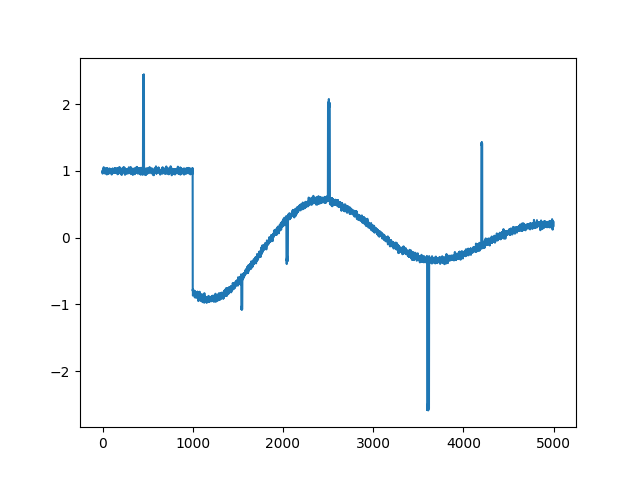
\includegraphics[width=25em]{func_60_tvd_01.png}

\begin{minted}[fontsize=\footnotesize]{python}
import numpy as np

eps = 1e-6
mu = 50.0

def phi_tv(x):
   return np.sum(np.abs(np.diff(x)))
   
def phi_atv(x):
   return np.sum(np.sqrt(eps + np.power(np.diff(x),2)) - eps)
   
def f(u):
   return np.sum(np.power(u-xcor, 2)) + mu*phi_atv(u)

print (phi_tv(xcor))
print (phi_atv(xcor))
\end{minted}

\begin{verbatim}
155.63025715999999
155.8936302273509
\end{verbatim}


\begin{minted}[fontsize=\footnotesize]{python}
u0 = np.zeros(len(xcor))
print (f(u0))

from scipy.optimize import minimize, Bounds, SR1, BFGS

opts = {'maxiter': 400, 'verbose': 2}

res = minimize (fun=f,
                x0=u0,
                options=opts,
                jac='2-point',
                hess=BFGS(),
                method='trust-constr'
                )

plt.plot(range(5000), res.x)
plt.savefig('')
\end{minted}

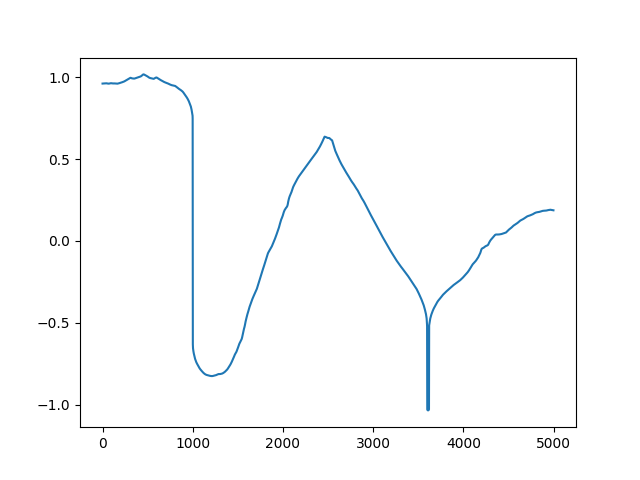
\includegraphics[width=25em]{func_60_tvd_02.png}



\inputminted[fontsize=\footnotesize]{python}{tvd.py}


Kaynaklar

[1] {\em ROF and TV-L1 denoising with Primal-Dual algorithm}, 
    \url{https://github.com/znah/notebooks/blob/master/TV_denoise.ipynb}

[2] {\em An introduction to continuous optimization for imaging}, 
    \url{https://hal.archives-ouvertes.fr/hal-01346507/document}

\end{document}



